\chapter{Geospatial Simulation Using Agent-Based Cellular Automata}
\label{chap:c4}

Understanding complex dynamics of our society and the environment we live in can give direction to solve social issues and contribute to global sustainability. Therefore, we study the problem of geospatial simulation in this chapter. Firstly we describe the agent-based cellular automata model, which is used for our simulation. Then we show that graph processing frameworks are adequate for large scale geospatial simulation, and propose a simulation algorithm. At the end the implementation details are given.

\section{Background of Simulation Models}

The geo-informatics with spatial and temporal data have assisted the investigation and modelling the environmental systems. Simulations are performed depending on different scenarios and objectives. Mobile entities such as vehicles and people move along their trajectories over a given space and time span. Simulations such as traffic simulation and pedestrian simulation are appropriate for these scenarios. 

Mathematical models in macroscopic simulation of this kind of behaviour have been studied for decades. However this approach is inappropriate to capture details as compared to the models that simulate in microscope, such as cellular automata or agent-based model. A profound impact on the whole system may be caused by a perturbation of an agent's action that leads to cascading effects\cite{suzumura2014towards}.

Cellular Automaton (CA) is a discrete spatio-temporal model, which is widely used in simulation of various real-world systems, such as social simulation. Cellular Automata consist of a regular grid of cells, each of which is in one of finite states. Each cell has a set of cells as \textit{neighborhood}, which is spatial relative to the cell. Each cell is assigned with an initial state. The next state of a cell is determined by some fixed rules depending on the current state of itself as well as its neighborhood. Typically the rule for updating the state of cells is same for every cell and does not change over time, and is applied to all cells simultaneously.

A typical example is two-dimensional cellular automata as a sheet of graph paper, in which each square represents a cell with its state and the rules to follow. The neighborhood is usually adjacent cells. The most common neighborhoods shown in Figure~\ref{fig:Neighborhood} are the von Neumann neighborhood, which is the four orthogonally adjacent cells, and Moore neighborhood, which is the eight surrounding cells. For example, the state of a cell is either white or black and the next state is determined by the dominant color of the neighborhood.

\begin{figure}
  \begin{center}
    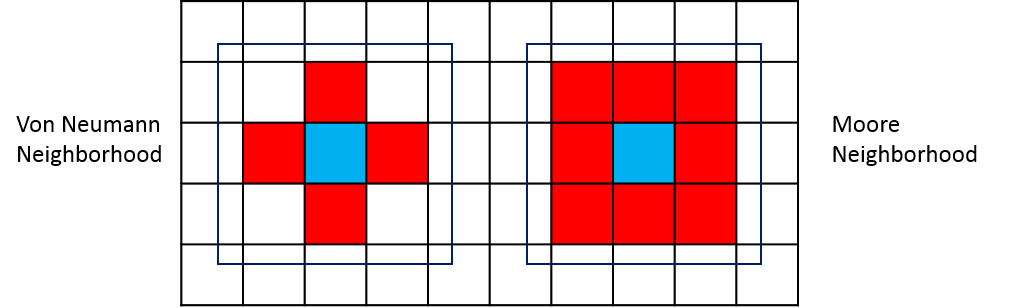
\includegraphics[width=\textwidth]{Neighborhood.png}
    \caption{Von Neumann neighborhood and Moore neighborhood}
    \label{fig:Neighborhood}
  \end{center}
\end{figure} 

Agent-based model (ABM) is a computational model for simulating the actions and interactions of multiple agents. An agent is an autonomous entity with self-contained program that is capable to perceive, decide and react on the environment. Agent-based model gives explanatory view on the collective behaviour and the effects of agents on the system as a whole. Agent-based model is a microscale model, which simulates the simultaneous actions and interactions of multiple agents to re-build or predict the occurrence of complicated phenomena. The process is reflection from micro level of the system to macro level, as the simple behavioural rules of agents lead to complicated behaviour of the system. ABM is able to represent and simulate more complicated and dynamical systems than CA.

Agent-Based Cellular Automata (ABCA)\cite{sudhira2005framework} is an integration of CA and ABM, which is capable to represent both spatio-temporal and agent dynamics. CA offsets the limitation of ABM to express the topology or the spatial relationships in the geographic perspective, and ABM brings the dynamics. In ABCA, agents are used to simulate the geographic objects in two-dimensional Euclidean space, so the definitions of the objects are points, lines and polygons. Agents move inside cells that define the transition rule. A cell reflects its local situation, and the collective effects of the cells contribute to observation as a whole.

ABCA is adequate for mobile-agent-based simulation, as interactions of agents are local in a cell. The parallel distributed computing system is ideal to execute this kind of simulation with large-scale datasets. In \cite{suzumura2012highly}, highly scalable X10-based agent simulation  platform XAXIS was used to simulate millions of agents in traffic flow simulation.

When geospatial simulation runs in Agent-Based Cellular Automata, a virtual space is composed of an array of cells, in which autonomous agents move around. When an agent goes beyond the border of its current cell, it migrates to the adjacent cell. The state of the cell changes with respect of to the agents inside it. 

\section{Simulation in Graph Processing Framework}

With the nature of the model, Agent-Based Cellular Automata is able to run on distributed systems like graph processing frameworks by partitioning the virtual area on distributed machines. Each machine has a set of cells, in which agents move round.

The simulation is pretty straightforward. The agents are initialized and the states of cells are based on their residing agents. Then the agents in the current cell update their locations. If the new location of a agent is beyond the area of the cell, it will migrate to the neighbor. Otherwise, the agent still resides in the current cell.

An agent becomes inactive and is removed when it can not update it location any more, and a cell becomes inactive when there is no active agent inside it. Therefore the simulation terminates when no agent exists and hence all cells are inactive.

The geospatial simulation using ABCA in GAS form is shown in Algorithm~\vref{alg:GAS_ABCA}. In the gather phase, the migrating agents from CA neighborhood of the current cell are gathered (line 1-3). The sum operation aggregates all migrating agents (line 4-5). In the apply phase, the vertex function merges its residing agents and the gathered agents, and clears all migrating queues (line 7-8). Then the vertex function updates the locations of its residing agents. If an agent moves beyond the current vertex, then the vertex function removes the agent and adds it to the corresponding queue (line 10-16). In the scatter phase, the vertex function activates itself, if it still has agents inside, and activates a neighbor, if the migrating queue of that neighbor is not empty (line 17-24).

The synchronization issue of ABCA is easily solved by using the synchronous engine. The algorithm can simulate with an arbitrary time interval specified by the user, and the synchronous engine guarantees the correctness of the spatio-temporal state. The collective effect of agents moving without conflict gives a view of the current situation in the macroscale.

	\begin{Algorithmus}[H]
	\label{alg:GAS_ABCA}
	\caption{Agent-Based Cellular Automata}	
	\begin{algorithmic}[1]
	\State //gather\_nbrs: IN\_NBRS
	\State \textbf{gather}$(D_u, D_{(u,v)}, D_v)$: 
	\State \textbf{return} agents $D_v.queue_u$
	\newline
	\State \textbf{sum}$(queue_a, queue_b)$: 
	\State \textbf{return} $queue_a \cup queue_b$
	\newline
	\State \textbf{apply}$(D_u, gathered\_agents)$:
	\State $D_u.queue_u \leftarrow D_u.queue_u \cup gathered\_agents$
	\State $\forall v \in u.neighbors, D_u.queue_v \leftarrow \emptyset $
	\State u.updateAgentsLocation()
	\For{agent $a$: $gathered\_agents$}
		\If{$u \neq a.destination$}
			\State $v \leftarrow a.destination$
			\State $D_u.queue_u \setminus \{a\}$
			\State $D_u.queue_v \cup \{a\}$
		\EndIf
	\EndFor
	\newline	
	\State //scatter\_nbrs: OUT\_NBRS
	\State \textbf{scatter}$(D_u, D_{(u,v)}, D_v)$: 
	\If{$D_u.queue_v \neq \emptyset$}
		\State 	Activate($v$)
	\EndIf
	\If{$D_u.queue_u \neq \emptyset$}
		\State 	Activate($u$)
	\EndIf
	\end{algorithmic}
	\end{Algorithmus}

\section{Implementation}

\subsection{Agent}

In our implementation, agents are simplified to points, which can be different, e.g. a shaped objects in other scenarios. An agent has its current coordinates and status as attributes, and agent updates its next coordinates according to the rule expressed in \textit{UpdateLocation()} method.

\begin{Listing}[H]
\begin{lstlisting}
enum AgentStatus { Unstarted = 0, Moving, Stopped };

class Agent
{
//methods
public:
	bool UpdateLocation();
//attributes		
public:
	double x;
	double y;
	AgentStatus agent_status;
};
\end{lstlisting}
\caption{Agent}
\label{lst:Agent}
\end{Listing}

\subsection{Cellular Automaton}

A cellular automaton should know its geographical space and the IDs of the neighbors, and it uses a vector of agent to hold inside agents and a map to hold the agents that migrate to the neighbors. Moore neighborhood is chosen to express the topology in our implementation. 

\begin{Listing}[H]
\begin{lstlisting}
class CellularAutomata
{
//attributes	
public:
	double space_top;
	double space_bottom;
	double space_left;
	double space_right;	
	vector<graphlab::vertex_id_type> neighbor_id;	
	vector<Agent> agents;
	map<graphlab::vertex_id_type, vector<Agent>> agents_to_target;
};
\end{lstlisting}
\caption{CellularAutomaton}
\label{lst:CellularAutomaton}
\end{Listing}

%\subsection{GAS Functions}